\documentclass[10pt,twocolumn]{article}
\usepackage{cite}
\usepackage{amsmath,amssymb,amsfonts,amsthm}
%\usepackage[full]{textcomp}
%\usepackage{fdsymbol}
%\usepackage{newtxtext,newtxmath}
\usepackage{multicol}
\setlength{\columnsep}{0.75cm}
\usepackage{caption}
\usepackage{graphicx}
\usepackage{csquotes}
\usepackage{todonotes}

\def\BibTeX{{\rm B\kern-.05em{\sc i\kern-.025em b}\kern-.08em
    T\kern-.1667em\lower.7ex\hbox{E}\kern-.125emX}}
\usepackage{hyperref}
\usepackage[margin=1.75cm]{geometry}
%794.96999pt and 614.295pt
\usepackage[hpos=600,vpos=590,angle=0,scale=0.5]{draftwatermark}
\SetWatermarkText{Preprint}
\SetWatermarkScale{2.35}
\SetWatermarkLightness{0.5}
\SetWatermarkText{Preprint of preliminary work}

\newtheorem{theorem}{Theorem}[section]
\newtheorem{corollary}{Corollary}[theorem]
\newtheorem{lemma}[theorem]{Lemma}

%\graphicspath{{img/}}


\title{Finding Maximum Expected Value Payment Flows for Reliable and Redundant Overpayemtens of Bitcoin on the Lightning Network}


\author{Rene Pickhardt}
\begin{document} 
\maketitle

\begin{abstract}
We study the problem of optimal payment planning - e.g. dissection of payment flows - in payment channel networks like Bitcoin's Lightning Network.
While Minimum Cost flows have been shown to maximize the probability of a payment flow we observe that they do not have to be the same as the maximum expected value flow for delivered Bitcoin.
This is shown by a concrete counter example.
We further formalize the theory of finding flows that maximize the expected value of delivered Bitcoin.
This yields the \texttt{plus one}-algorithm that can find the maximum expected value payment flow.
The \texttt{plus x}-algorithm is presented as an approximation with faster runtime and nicer properties for the participants of the network.
Both algorithms can be used to plan a redundant overpayment where the overpayment ist made at least so redundant that the expected value that will be delivered meets the amount that the sender is asked to deliver in the invoice.
Relying on a protocol upgrade to support secure redundant overpayemts with the techniques presented in this paper payments would on average settle with one round of concurrent network round trips.
\end{abstract}

\section{Introduction}
Delivering satoshis on Bitcoin's Lightning Network is a burden for the sending node as it does not know how the capacity of remote channels is split into liquidity owned by each peer.
Thus selecting channels to route the payment is limited by this uncertainty.
Prior work \cite{pickhardt2021security} has used probability theory to quanityfy the uncertainty about the remote liquidity in an information theoretic sound way.
The authors haver in particular indicated that the problem of planning a payment that reduces the uncertainty is equivalent to a payment that maximizes the successprobability of complete delivery.
Followup work by the same authors \cite{pickhardt2021optimally} demonstrated that the optimization problem can be understood as a minimum cost flow problem with a convex seperable integer cost function.
After piecewise linearization this can be modelled as a linear minimum cost flow problem and be computed sufficiently quick \cite{pickhardt2022}.

However the work of the authors lacks an important observation. If a recipient of a payment issues an invoice for the amount $a$ and the payment flow $f$ has a success probability of $s(f)\leq 1$ then the expected amounts of sats to be delivered on the first attempt will on average be lower than the amount $a$.
This means that some of the planned onions will return to the recipient who will now in a round based payment loop compute new mininum cost flow problems and - even worse - have additional network roundtrips and sending of onions which will increase the latency of the entire payment process and keep remote liquidity of the previously successful onions locked and not usable for other participants of the network.

It obviously makes sense to plan a payment flow which has an expected value of delivered satoshis that is as least as the amount $a$ of requested satoshis by the recipient in the invoice.
As the minimum cost flow already has the highest probability we know that we can only achieve this with the help of redundant overpayments.
This technique has been proposed and requested several times in the past \cite{bagaria2020boomerang,rahimpour2021spear,corallo2023,riard2023}.
However it has only been studied in an ad hoc way - with arbitrary splits of the payment amount. But even in such conditions it was demonstrated that it can reduce the \texttt{locked liquidity} times \texttt{time} metric. 
So far no systematic study exists that shows what reasonable amount of liquidity should be allocated by the sending node and how exactly the payment should be planned to optimize the quick delivery of the payment.

As indicated we believe an optimal payment planning with redundant over payments should create a payment flow that has at least an expected value of delivered satoshis as the amount of sats requested in the invoice.
This paper will systematically show why the minimum cost flow problem is not suitable to address that question and present two greedy heuristics that can be used to find a payment flow with such an expected value.
If higher services level agreements or confidence is necessary the algorithms can be extended to plan flows with even higher expected values.
The only open question of this research is weather flows with less required allocated liquidity exist that have the same expected value.

\section{Expected value of the delivered payment amount through a remote channel}
Let $e=(u,v,c)$ be a remote payment channel between nodes $u$ and $v$ with an integer capacity of $c \in\mathbb{N}$.
The fact that the channel is remote means that we have uncertainty about the existing liquidity that $u$ has in the channel which consequently means we do not know how many sats we can forward in a routing request from $u$ to $v$.
Following the information theoretic frame work of \cite{pickhardt2021security} we can express the probability to forward $a$ satoshis from $u$ to $v$ as
\[
P(X\geq a)
\]

\subsection{Atomic Payment Delivery strategy}

Sending $a$ satoshis on this channel one can expect
\[
E[a] := a\cdot P(X\geq a)
\]
satoshis to be forwarded on average.
Assuming a uniform distribution the expected value is defined by the follwoing function:
\[
E[a] = a\cdot\frac{c+1-a}{c+1}
\]
the maxium can be found by looking at the derrivative $\frac{\partial E[a]}{\partial a} = \frac{c+1 -2a}{c+1}$.
This expression takes the value $0$ at $a=(c+1)/2$ and the expected number of sats to arrive will be: $(c+1)/2 \cdot (1 - \frac{c+1}{2\cdot(c+1)}) = \frac{c+1}{4}$. We have plotted the uniform case and the bimodal distribution\footnote{The bimodal model is recently being added to LND. c.f.: \url{https://lightning.engineering/posts/2023-03-29-lnd-0.16-launch/}} in figure~\ref{fig:atomicPayment}:

\begin{figure}[htpb]
  \center
  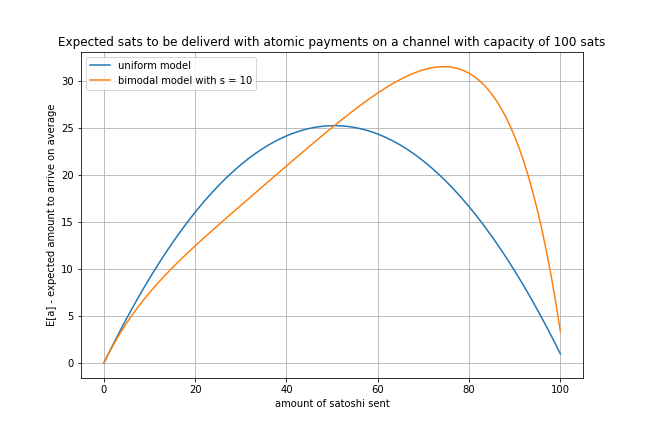
\includegraphics[width=0.45\textwidth]{img/atomicPaymentSingleChannel}
  \caption{Expected Value of sats to be delivered for various amounts with atomic single payment delivery strategy on a channel with capacity of $100$ for a uniform distribution and abimodal distribution for the uncertainty of the liquidity as a prior.}
  \label{fig:atomicPayment}
\end{figure}

\subsection{Optimal Payment Delivery Strategy}
Let $a$ be the liquidity we have available to send.
We do not have to send the amount atomically in one payment request.
Even on the same remote channel we can make several forwarding requests of smaller amounts.
Let us assume we peel of $1$ satoshi then the expected amount that is delivered could be described via:
%TODO: WHY?!? symmetry!
\[
E[a-1,1] = (a-1)\cdot P(X\geq a-1) + 1 \cdot P(X\geq a)
\]
We claim that $E[a-1,1] \geq E[a]$ and do so by prooving the following lemma:

\begin{lemma}
\label{lemma}
Atempting to deliver the avalable liquidity $a$ atomically in a single payment attempt has a lower or equal expected value of delivered satoshis than the strategy that peels $1$ satoshi off and sends two payments of size $a-1$ and $1$.
\end{lemma}
\begin{proof}
We note that for any prior probability distribution we have
\[
P(X\geq a-1) \geq P(X\geq a)
\]
Thus we have:
\begin{equation}
\begin{split}
E[a-1,1] & = (a-1)\cdot P(X\geq a-1) + 1 \cdot P(X\geq a) \\
 & \geq (a-1)\cdot P(X\geq a) + 1 \cdot P(X\geq a) \\
 & = a \cdot P(X\geq a) \\
 & = E[a]
\end{split}
\end{equation}

This shows that:
\[
E[a-1,1] \geq E[a]
\]

\end{proof}

With this lemma we can deduct an importat corollary:

\begin{corollary}
\label{corollary}
Let $a$ be the available liquidity that can be used to deliver a payment. Then splitting the liquidity into $a$ parts of one unit will yield the highest expected value of liquidity to be delivered through the remote channel.
\end{corollary}

\begin{proof}
We note that $E[a-1,1] = E[a-1] + 1\cdot P(X>=a)$. We can thus apply the lemma again to the term $E[a-1]$ and realize that $E[a-2,1] \geq E[a-1]$. Of course we can continue to increase the expected value by peeling of 1 unit. If we do so we get:
\[
E[\underbrace{1,\dots,1}_{\texttt{a times}}] = \sum_{i=1}^a P(X\geq i)
\]
\end{proof}

For the uniform distribution we can use the gausian sum formular to analytically compute the expected value of the optimal strategy to make $a$ payment requests of $1$ unit each.
We thus have the following formular for the expected satoshis that can be delivered:
\begin{equation}
\label{eq:expvalue}
E[\underbrace{1,\dots,1}_{\texttt{a times}}] = a - \frac{a(a+1)}{2\cdot(c+1)}
\end{equation}

Again one can compute the derrivative with respect to $a$ which has the form:
\[
\frac{2c-2a+1}{2c+2}
\]
For $a=c+\frac{1}{2}$ the derrivative takes the value $0$.
As the function is only defined for $a\in\{0,1,\dots,c-1,a\}$ the maximum of the function is taken at $a=c$
Putting this into equation \ref{eq:expvalue} we see that the expected value is $c-\frac{c(c+1)}{2(c+1)} = \frac{c}{2}$  which is also being depicted in figure \ref{fig:optimalPaymentSingleChannel} where we again have also plottet the expected value for the bimodal model:

\begin{figure}[htpb]
  \center
  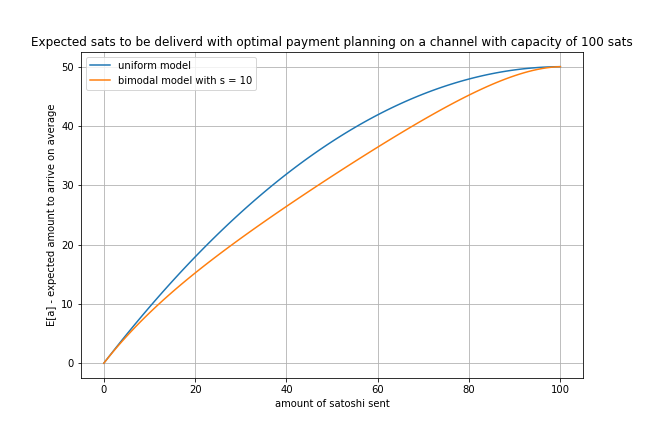
\includegraphics[width=0.45\textwidth]{img/optimalPaymentSingleChannel}
  \caption{Expected Value of sats to be delivered for various amounts of sendable liquidity with the optimal payment delivery strategy on a channel with capacity of $100$ with a uniform distribution and a bimodal distribution as a prior to encode the uncertainty about the liquidity.}
  \label{fig:optimalPaymentSingleChannel}
\end{figure}

\section{Expected Delivery Value of paths through a network}
The observations and results from the previous section easily generalize to paths instead of channels.
As described in \cite{pickhardt2021security} the success probabilty for a path can be described as the joint distribution of the success probability for its channels.
Thus each path with $n$ channels has a success probability which can be described as
\[
P(\vec{X} \geq a) = \prod_{i=1}^n P(X_i \geq a)
\]

Also the expected value of delivered satoshis is the probability of the path times the amount that is allocated to the path.
In particular lemma \ref{lemma} and the corollary \ref{corollary} do also hold true for paths since we prooved the validity for an arbitraty probability distribution.

\section{Finding a payment flow with at least a certain expected value.}

The fact that the flow that maximes the expected value that can be delivered if $a$ satoshis of liquidity are provided has to consist of $a$ paths that sent $1$ satoshi each can be used to provide a greedy algorithm to compute the maximum expected value payment flow.
Assuming a network with the sender $S$ and a recipient $R$ in which $S$ wishes to use $a$ satoshis of liquidity to plan a payment with maximum expected value of satoshis to arrive at $R$.
The greedy algorithm works in $a$ rounds of augmenting paths to the final payment flow that maximizes the expected value of delivered satoshis.

Initially the allocated flow is $f=0$ and we create the residual Network $R_f$.
For each arc $a_{ij}$ in the original network we add an arc $r_{ij}$ to te residual network $R_f$.
The cost $c(r_{ij})$ for the arc $r_{ij}$ is computed as:
\[
cost(r_{ij})=-\log(P(\vec{X} \geq f_{ij} + 1)
\]
If an arc has already flow allocated in a direction $(i,j)$ we add an addtional arc in the opposite direction $(j,i)$ with the following cost:
\[
cost(r'_{ji}) = -\log\left(\frac{1}{P(\vec{X}\geq f_{ij}}\right)
\]
This cost is necessarilly negativ and can be interpreted as a discount one is given to unsaturate the arc in the next round.

The algorithm will in $a$ rounds repeat the following steps
\begin{enumerate}
\item Compute the residual network.
\item Find a shortest path $p$ with total cost $C$ from $S$ to $R$.
\item Update the flow $f$ by augmenting the path $p$. Augmenting means that the flow of the arcs along the path is increased by $1$ Satoshi (or reduced in the opposite direction if the arc had negative cost).
\item Updated the expected value by adding $2^{-C}$ to the current expected value.
\end{enumerate}

We do not know yet if that greedy heuristic finds the flow that maximizes the expected delivered payment value for a fixed amount of available liquidity.
However it has several downsides other downsides in practice:
\begin{enumerate}
\item The runtime is $O(a\cdot n^3)$ because we have to solve $a$ Bellmann Ford problems.\footnote{This may be drastically reduced as a new algorithm to solve single source shortest path problems in near linear time has emerged \cite{bernstein2022negative}}
\item On payment channel networks like the Lightning Network we would not wish to send out $a$ different requests to deliver $a$ (or fewer) satoshis.
\end{enumerate}

However the algorithm can easily be adopted to an approximation.

\section{Quick Approximation to find flows with at least a certain expected value.}
Instead of finding the mostlikeli $1$ sat path and augment $1$ sat to the payment flow one could augment $x$ satoshi paths in each round.
The cost formulars in the residual network are easily updated to

\[
cost(r_{ij})=-\log(P(\vec{X} \geq f_{ij} + x)
\]
while the cost for the backward edge stays the same:
\[
%cost(r'_{ji}) = -\log\left(\sum_{i=0}^{x}\frac{1}{P(X \geq f_{ij} - i)}\right)
cost(r'_{ji}) = -\log\left(\frac{1}{P(\vec{X} \geq f_{ij})}\right)
\]
The algorithm will now only need to solve $a/x$ shortest path problems.\footnote{In particular the topology of the network does not change too much during each round so that a $D^*$ style algorithm \cite{stentz1997optimal} may be useable.}
The new algorithm has some nice properties.
First the structure of the cost function does not matter.
In particular the cost function may be non linear so that the base fee is not a problem.
At the same time even if routing fees are added to the cost function the algorithm does not globally minimize them as a minimum cost flow would do.
Generally one does not wish to send out too many concurrent payments so the value of $x$ can be choosen with respect to $a$ and the number of concurrent payments one wishes to conduct.

\subsection{Planning of redundant overpayments}
The idea of sending redundant overpayments to improve reliability of payment channel networks is not novel and has been proposed in \cite{bagaria2020boomerang,rahimpour2021spear}.
It has also frequently been discussed by developers \cite{pickhardt2022,riard2023,corallo2023}.
However so far no solution to the problem of how to plan a redundant overpayment and by which amount it should happen has been proposed.
Both of the above algorithms produce a rather natural way to planning a redundant overpayment.
In each round of the exact and the approximate algorithm the expected value of delivered satoshis for the current flow is updated.
If some sender $S$ wishes to deliver the amount $a$ and decides to send chunks of size $x$ one can continue to augment the flow until either no new path can be found to augment the flow (meaning the problem is infeasible) or until the expected value of delivered satoshis $e = E[\underbrace{x,\dots,x}_{\texttt{k times}}]$ is larger than the amount $a$ that the sender wishes to send. In that case $k$ is the total number of concurrent payment requests that will be sent out and $r = \frac{k\cdot x}{e}$ is the redundancy factor.



\section{Comparison to Min Cost Flows}
Prior research \cite{pickhardt2021optimally} claimed that optimally reliable payment flows are discovered by solving a minimum cost problem in which the cost function parameterized the information content - sometimes refered to the uncertainty cost - of each channel.
The authors showed that minimizing the uncertainty cost is equivalent to maximizing the probability of the resulting flow.
While standard algorithms exist to disect a flow into paths we have indicated that the actual disection and planning of payments has an impact on the expected amount of satoshis that will be delivered.
The authors did not make a statement weather minimum cost flows that maximize the total probability of the flow would also maximize the expected amount of delivered satoshis if the payment flow is disected optimally.

In particular we will now provide an example network in which the minimum cost flow - even with optimal disection of the flow into paths - will have a lower expected value of delivered satoshis than the flow that our exact \texttt{plus one}-algorithm finds to maximize the expected number of deliverd sats.
The network is described in the following diagram \ref{fig:counterExample}

\begin{figure}[htpb]
  \center
  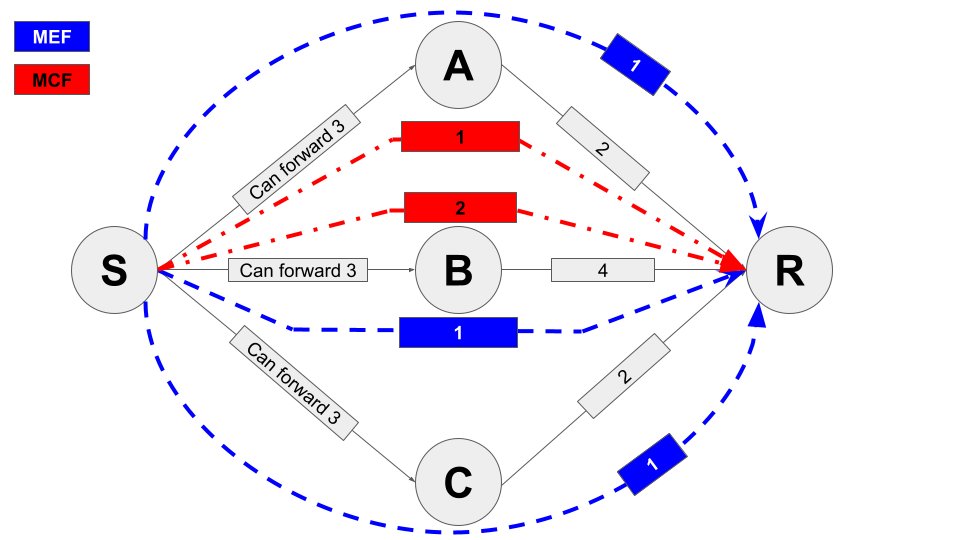
\includegraphics[width=0.45\textwidth]{img/counterExample}
  \caption{Network in which the Minimum Cost flow does not maximize the expected amount of satoshis to be deliverd}
  \label{fig:counterExample}
\end{figure}

Assume the sender $S$ has enough liquidity in all channels to routing nodes $A,B,$ and $C$ and wishes to allocate $3$ satoshis of local liquidity to plan a payment via a payment flow.
For simplicity assuming a uniform distribution of the liqudity one minimum cost flow will send 1 sat via $S \rightarrow A \rightarrow R$ with a probability of $\frac{2}{3}$ and send the other $2$ sats via $S \rightarrow B \rightarrow R$ with a probability of $\frac{3}{5}$. This results in a total probability for the payment to settle of $P(mcf)=\frac{2}{5} = 0.4$.
The expected value by sending out $3$ single sat onions is computed as:
\[
E[mcf] = \frac{2}{3} + \frac{4}{5} + \frac{3}{5} = \frac{31}{15}
\]

However using the \texttt{plus one}-algorithm we find the maximum expectation value flow (mef) that sends $1$ satoshi across each of the $3$ disjoint paths.
The expectation value is computed as:
\[
E[mef] = \frac{2}{3} + \frac{4}{5} + \frac{2}{3} = \frac{32}{15}
\]

This flow expects to deliver $\frac{1}{15}$ sats more than the minimum cost flow.
To see that the discussed flow is not the minimum cost flow we comput its likelihood as:
\[
P(mef) = \frac{3}{3} \cdot \frac{4}{5} \cdot \frac{2}{3} = \frac{16}{45} = 0.3555\dots < 0.4 = P(mcf)
\]
Thus we conclude that while computing minimum cost flows has shown impressive results to payment delivery on the lighting network they do not maximize the expected amount of delivering payments and also do not naturally lead to planning strategies that allow for redundant overpayments.

\section{Experimental Setup}
We use a simulation to test the proposed algorithm.
With a current snapshot of the Lightning Network from the gossip protocol we initiate the liqudity following a uniform distribution.
Using a uniform distribution again we randomly generate $1000$ payment pairs.
Using the available liquidity information we compute a maxflow for each pair to know how many sats could actually be delivered.
Knowing that the piecewise linearized mininmum cost flow as well as the new algorithm produce approximations we take half of the theoretically possible amount as requested payment amount for each payment pair.
On the same snapshot of the oracle network (in which the liquidity is known) we try to deliver the payment through a payment loop using the mininum cost flow approach as well as the redundant overpayment approach.
We track the histrogram of necessary rounds of flow computation as well as the \texttt{locked liquidity} times \texttt{time} (LLT) metric.

\section{Evaluation}

\section{Related Work}
The authors of \cite{aneja1980maximal} have studied flows that maximize the expected value in networks with arcs that have failure probabilities.
However the failure probabilities in that work were constant per arc and not depending on the level of saturation as in our case.
Similarly the authors of \cite{sancho1988maximum} studied the maximum expected flow problem in reliable networks but used a fixed probability for each path to encode the reliablity.
For reliable networks - e.g. networks where a fixed failure probabliity for each arc exists - it is known that the computation of the maximum expected flow is computationally hard but methods for speeding up the discovery of the flow exist \cite{sharma2013speeding}.

\section{Conclusion and open questions}
We demonstrated once more the usefulness of redundant overpayments and encourage the Lightning Network developer community to add one of the previously proposed cryptographic protocols to the BOLTs.
We show that using the new techniques we can settle $x\%$ of payments with only one round of concurrent network roundtrips.

It remains open to find an optimal maximum expected value flow algorithm and to proof how close our greedy heuristics are to the optimum.
Another question that needs more study is to understand how high the expected value should be as a multiple of the requested amount to statistically ensure delivery of payments within one round of concurrent network roundtrips.
Similarly we need to study how many shards and what shard size is useful.

\bibliography{paper}
\bibliographystyle{plain}
\end {document}
